\section{Introduction}
\label{sec:intro}
The Standard Model (SM) has been proved to be an accurate description 
of production of elementary particles observed so far. The interaction of W bosons
with photons is particularly important as a important test of self coupling 
of these bosons as predicted by non-Abelian gauge group of electroweak sector. Precise measurements of diboson properties and cross 
sections are a crucial step towards understanding the production of major 
backgrounds of Higgs boson searches at LHC. 

In this analysis note we report the analysis of inclusive $W\gamma + X$  processes  
using  leptonic decays of $W\to \ell\nu$ where $\ell = e, \mu$. 
The $W\gamma$ productions at tree level can be represented by Feynman diagrams in 
Figs.~\ref{fig:feynman_wg}~and~\ref{fig:feynman_zg} 
as three processes: initial state radiation (ISR) where a photon is produced from one of 
the incoming partons, final state radiation (FSR) where a photon is radiated off one of 
the charged leptons from the $W$ boson decay, and finally when a photon is produced in 
$s-$channel via TGC $WW\gamma$ for $W\gamma$ production.  The last process is allowed only for $W\gamma$g production in the SM, as there are no neutral TGC in the SM.
\begin{figure}[htb]
\begin{center}
{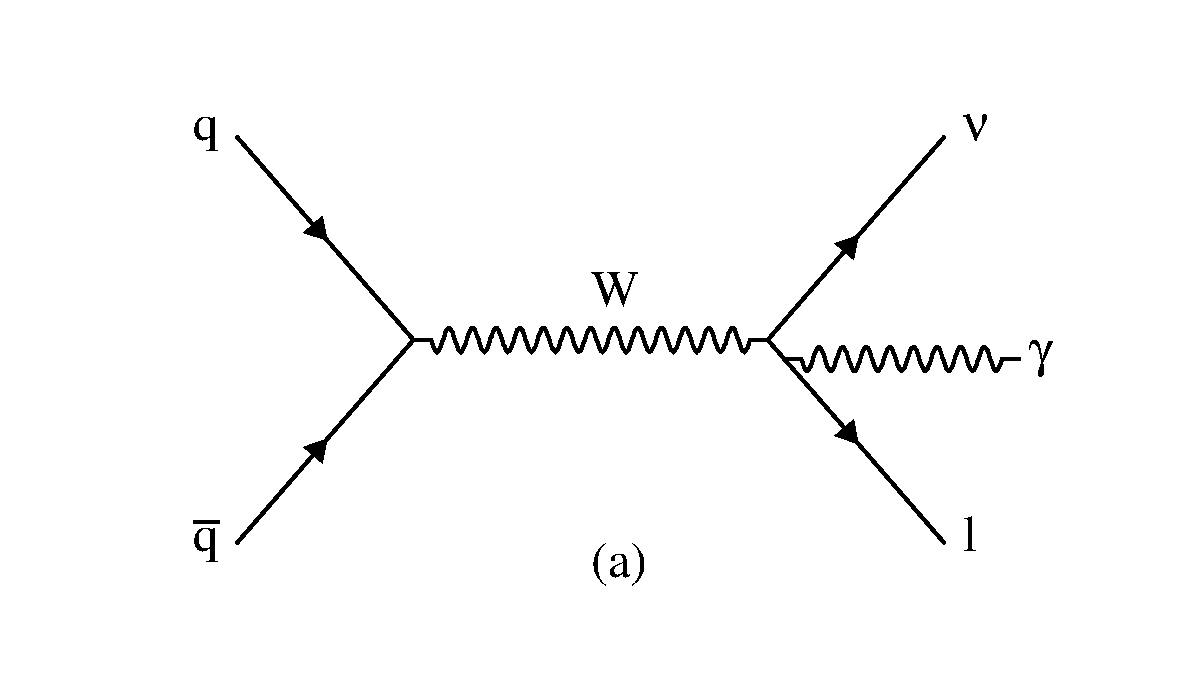
\includegraphics[width=0.49\textwidth]{figs/wg_fsr}}
{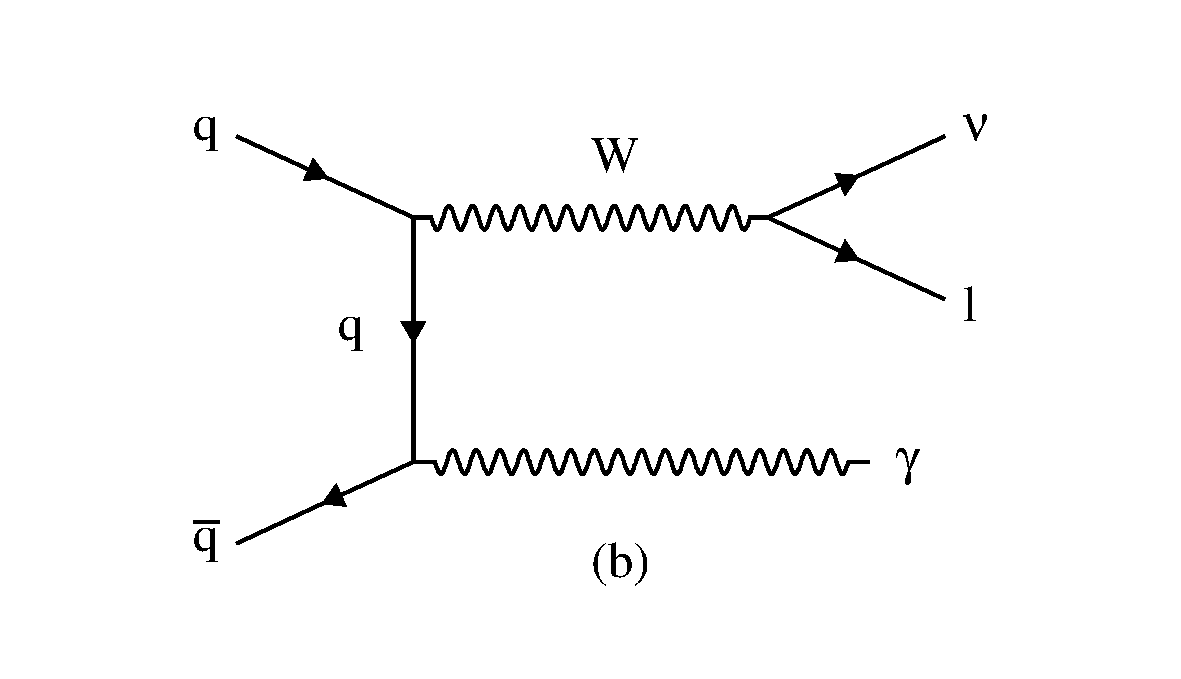
\includegraphics[width=0.49\textwidth]{figs/wg_isr}}
{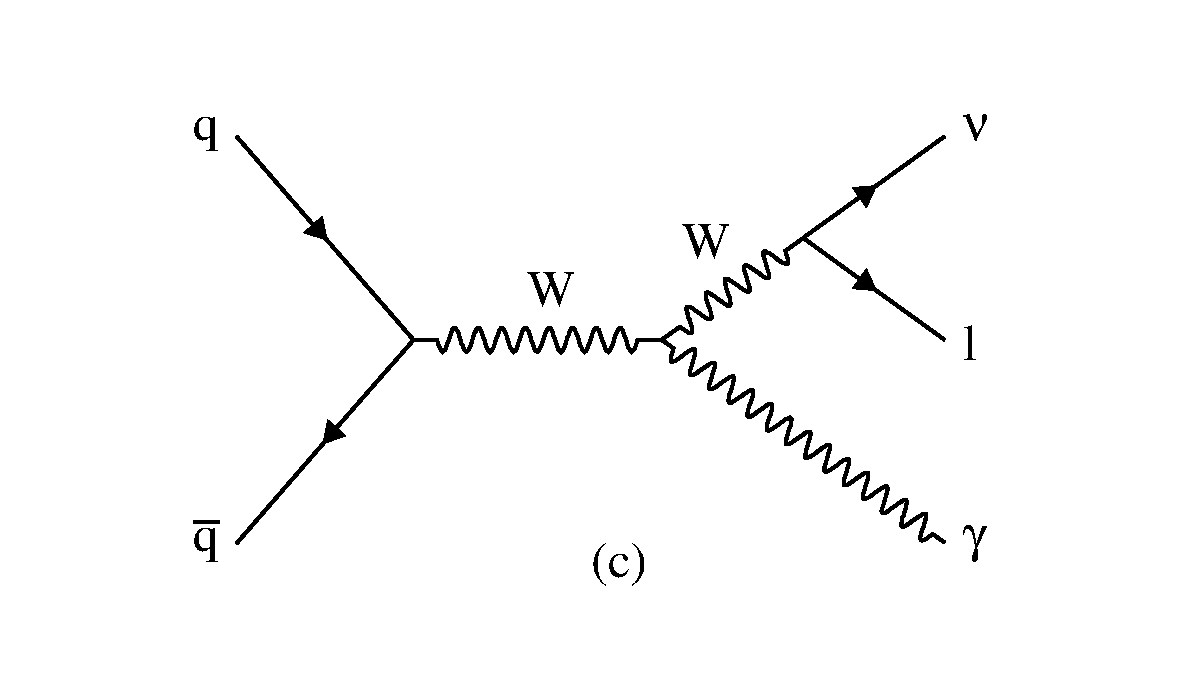
\includegraphics[width=0.49\textwidth]{figs/wg_wwg}}
\caption{Feynman diagrams of the W$\gamma$ production via 
final (a) and initial (b) state radiation and via WW$\gamma$ 
trilinear gauge coupling (c).}
\label{fig:feynman_wg}
\end{center}
\end{figure}

